%!TEX ROOT=../dissertation.tex

\chapter{ČTK Dataset Analysis and Postprocessing}
\label{chap:dataset}

Through the methodology described in chapter~\ref{chap:ctk}, we have collected a set of raw claims and samples of their veracity labelling.

This chapter performs the exploratory analysis of the collected dataset, structured as described with Figure~\ref{fig:er}, and describes our methods of \"{flattening} it into a single text file that is easy to parse. Consecutively, we analyse the resulting dataset using several standard metrics and propose tools for its iterative refinement, ultimately leading to the current version of \textsf{ČTK} dataset, described and linked in~\ref{sec:dataset-latest}.

\begin{figure}[H]
\makebox[\textwidth][c]{{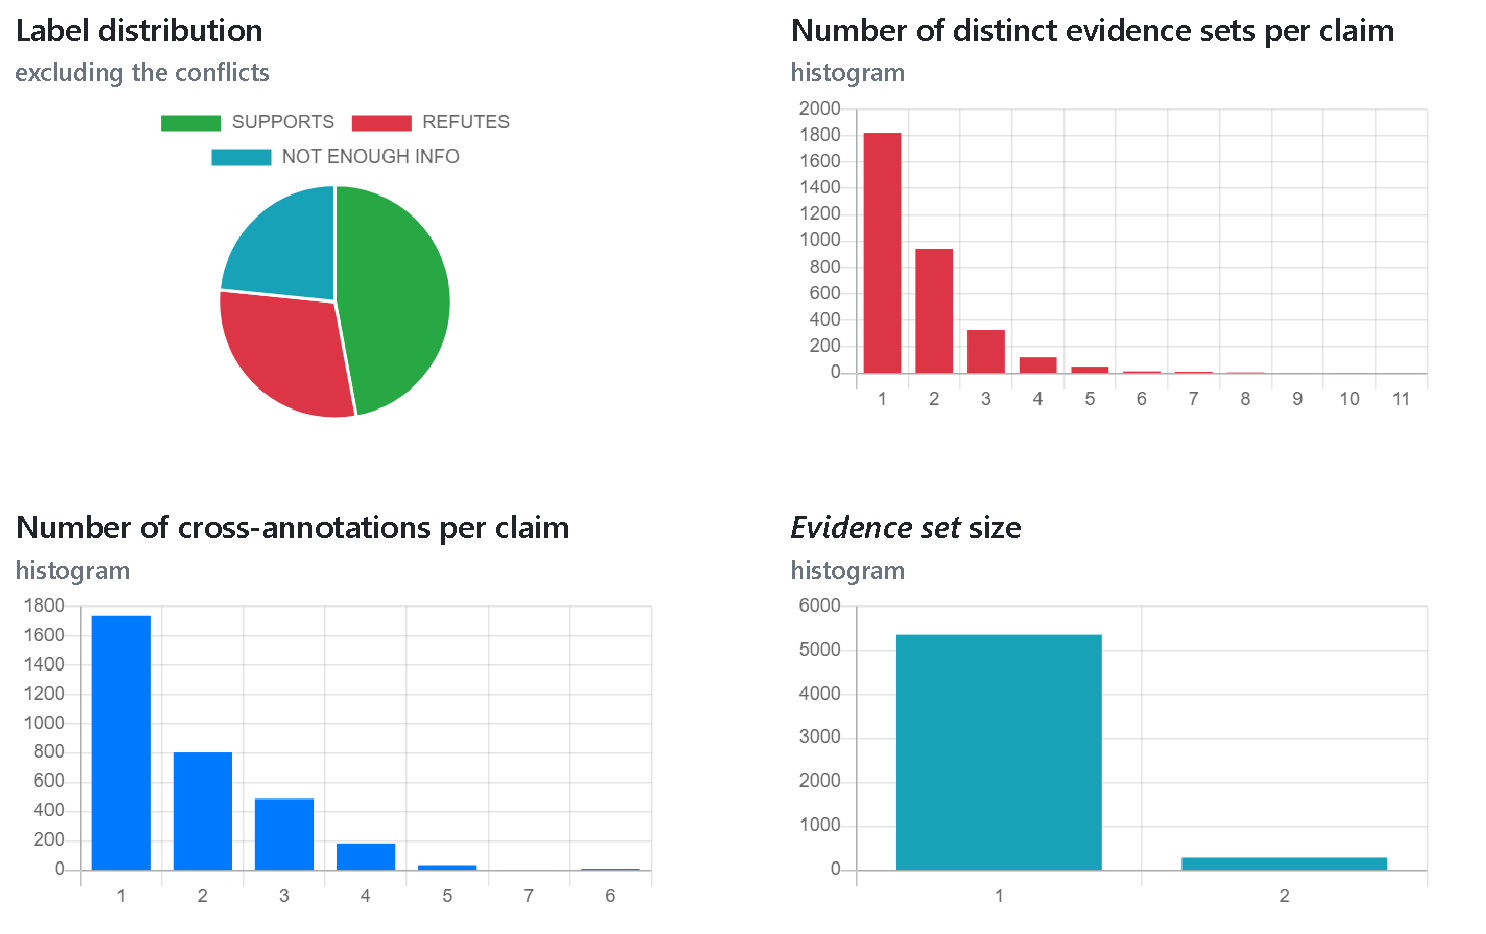
\includegraphics[width=16cm]{fig/dashboard.pdf}}}
\caption[Visualizations of properties of the collected dataset]{Visualizations of properties of the collected dataset, extracted from our interactive dashboard (Section \ref{sec:dashboard}) attached to this thesis.}
\label{fig:dashboard}
\end{figure} % zeleny graf

\section{Live Dashboards}
\label{sec:dashboard}
In order to provide our users with a comprehensible view into the resulting dataset and its properties, including the leaderboard of the most active annotators, we have implemented a dashboard of \textit{live} data visualizations. For the live data aggregations, we have mostly used raw \textsf{PHP} and \textsf{SQL}, for interactive and \ae{}sthetically pleasing plots, we have used the \textsf{Chart.js} library.

We have decided to disclose the dashboard (with supplementary labels in Czech) to our reader, so as to accompany the texts to follow, and to provide a legible statistical insight into the data collected by the methods listed in Chapter~\ref{chap:ctk}.

It can be found at \url{https://fcheck.fel.cvut.cz/site/statistics} and logged into using the \"{\texttt{testuser}} \textsf{SIDOS ID}.

\section{JSON Lines FCheck Export}
\label{sec:export}
For the purpose of \textit{flattening} the \textsf{FCheck} database with all of its relations and metadata to a single concise text file used on an input for our end applications, we have constructed a \textsf{JSONL API} at \texttt{https://fcheck.fel.cvut.cz/label/export}.

It takes the following arguments through its \textsf{HTTP GET} parameters:
\begin{enumerate}
    \item \texttt{shuffle} $\in\{\texttt{0},\texttt{1}\}$, defaults to \texttt{0}\\ decides, whether the dataset should be shuffled using the \textsf{MySQL}'s \dots\texttt{ORDER BY rand()}
    \item \texttt{evidenceFormat} $\in\{\texttt{text},\texttt{ctkId}\}$, defaults to \texttt{ctkId}\\
    if set to \texttt{text}, the full detokenized text of used \textsf{ČTK} paragraphs will be exported for evidence (preferred for NLI), otherwise, only the underscore-separated article and paragraph id will be given, s.a. \texttt{T201810060771501\_2} (preferred for DR)
    \item \texttt{summer} $\in\{\texttt{0},\texttt{1}\}$, defaults to \texttt{0}\\ decides, whether the first wave of annotations  should be excluded from the export, by default it is sorted by the source paragraph
    \item \texttt{fever} $\in\{\texttt{0},\texttt{1}\}$, defaults to \texttt{0}\\ switches to the \textsf{FEVER}-like output format (\ref{list:fever}), to ease the usage of \textsf{FCheck} data for experiments implemented to run with \textsf{FEVER CS} -- setting to \texttt{1} disables the other options for legacy reasons
\end{enumerate}

\subsection{ČTK dataset formats}
While much like~\cite{fever} we use the \textsf{JSONL} file type, which we deem appropriate for the fact verification datasets, we propose an alternate format for flattening the data points than that from Figure~\ref{list:fever}. In our case, we argue to suppress all the auxiliary information except the \db{Claim} \texttt{id} to refer back to the \ref{fig:er} representation of data, following the KISS\footnote{\"{Keep It Simple, Stupid!}} and YAGNI\footnote{\"{You Ain't Gonna Need It.}}~\cite{jeffries2001extreme} design principles.

While this interpretation of the \textit{labeled-claim} datapoints is our current default, we also enable switching back to the \textsf{FEVER} format illustrated in~\ref{list:fever}, using the \texttt{fever} flag for backwards compatibility. This is particularly useful for reusing the model training procedures written for \textsf{FEVER CS}. 

We demonstrate the two types of \db{Evidence} representation in Figures~\ref{list:fcheck-ctkid} and~\ref{list:fcheck-text} -- \texttt{text}  is meant for the training and validation of the NLI models (Chapter~\ref{chap:nli}), whereas \texttt{ctkId} suits the Retrieval tasks. For the completeness, the \texttt{ctkId} consists of the \textsf{ČTK Archive} identifier and the paragraph 1-based index in the archived article, separated by underscore. Index 0 is reserved for the article headline as it may also be used for both tasks.

\begin{figure}[H]
\begin{lstlisting}[language=json]
{
  "id": 2500,
  "label": "SUPPORTS",
  "claim": "S Dejvickým divadlem spolupracoval Petr Zelenka.",
  "evidence": [
    ["T201111230392601_9"],
    ["T200708140695001_2"]
  ]
}
\end{lstlisting}
    \caption[Example of \textsf{ČTK} datapoint, \texttt{ctkId} evidence format]{Example \textsf{ČTK} \texttt{SUPPORTS} annotation with two possible evidence sets, each composed of one \textsf{ČTK} paragraph, using the \texttt{ctkId} evidence format.}
    \label{list:fcheck-ctkid}
\end{figure}
\begin{figure}[H]
\begin{lstlisting}[language=json,escapeinside={(*}{*)}]
{
  "id": 2500,
  "label": "SUPPORTS",
  "claim": "S Dejvickým divadlem spolupracoval Petr Zelenka.",
  "evidence": [
    ["Petr Zelenka vystudoval scenáristiku a dramaturgii na FAMU (*(\dots)*) V roce 2001 napsal pro Dejvické divadlo (*Příběhy*) (*obyčejného*) šílenství, za které získal Cenu Alfréda Radoka (*(\dots)*)"],
    ["(*(\dots)*) kterou Zelenka (*později*) (*režíroval*) i jako stejnojmenný film. V roce 2005 uvedl na dejvické (*scéně*) svou (*další*) hru Teremin. V (*současné*) (*době*) (*natáčí*) Zelenka osobitou verzi inscenace Dejvického divadla Karamazovi."]
  ]
}
\end{lstlisting}

    \caption[Example of \textsf{ČTK} datapoint, \texttt{text} evidence format]{The same example as~\ref{list:fcheck-ctkid} using the \texttt{text} evidence format, paragraphs were truncated using \texttt{(\dots)}}
    \label{list:fcheck-text}
\end{figure}
\begin{figure}[H]
\begin{lstlisting}[language=json,escapeinside={(*}{*)}]
{
  "label": "SUPPORTS",
  "claim": "S Dejvickým divadlem spolupracoval Petr Zelenka.",
  "context": [
    "(*(\dots)*) Petr Zelenka (*(\dots)*) napsal pro Dejvické divadlo (*(\dots)*)"
  ]
}
\end{lstlisting}

\begin{lstlisting}[language=json,escapeinside={(*}{*)}]
{
  "label": "SUPPORTS",
  "claim": "S Dejvickým divadlem spolupracoval Petr Zelenka.",
  "context": [
    "(*(\dots)*) kterou Zelenka (*(\dots)*) 2005 uvedl na dejvické (*scéně*) (*(\dots)*) "
  ]
}
\end{lstlisting}

    \caption[Example of \textsf{ČTK} datapoint, \texttt{nli} evidence format]{The same example as~\ref{list:fcheck-text} using the \texttt{nli} evidence format, paragraphs were truncated using \texttt{(\dots)}. Note that in this format we have 2 datapoints - one for each evidence set.}
    \label{list:fcheck-nli}
\end{figure}

Additionally, we introduce the \textsf{ČTK} \texttt{nli} format that is appropriate for training and testing the Natural Language Inference models in the Figure~\ref{list:fcheck-nli}, note that this format produces a different number of datapoints, one for every evidence set, listed as \texttt{context}.



\section{Cross-annotations}
\label{sec:cross-annotations}
In \textsf{FEVER} annotation labeling task \textsf{WF2}~\cite{fever}, the annotators were advised to spend not more than 2-3 minutes to find as many of the evidence sets as possible in the given dictionary (and even using a direct \textsf{Wiki} access), so that the dataset can later be considered \textit{exhaustive}, i.e., to boost its \textit{evidence recall}, which was later computed to be \textbf{72.36\%}.

With our \textsf{ČTK Archive} corpus, this is unrealistic, as it commonly contains an inconceivable number of copies for a single ground truth\footnote{Think, the proposition \"{Miloš Zeman is the Czech president}, which can be found in every \"{(\dots), said the Czech president Miloš Zeman.}}. So is the number of paragraphs in the \textit{mutated claim}'s knowledge scope, typically close to (see \tjednab{} and \ref{sec:knowledge-scopes} for reference) $\text{max}_{m^c}|knowledge(m^c)\cup knowledge(p) \cup\{p\}|=17$. Therefore, we proposed a different scheme: we advised every annotator to spend 2-3 minutes finding a \textit{reasonable} number of distinct evidence-sets, w.r.t. the time needed for a good reading comprehension. Furthermore, we randomly shuffled the set of all \textit{knowledge scope} documents using \textsf{PHP}'s \texttt{shuffle}\footnote{Which internally uses the Mersenne Twister pseudorandom number generator, for the completeness} before the start of every \tdva{} annotation.

As the annotators typically skim through the knowledge headlines in a top-first order, this made it difficult for two annotators to arrive to the same set of evidence-sets. To exploit that, we collected multiple \textit{cross-annotations} for each claim -- their distribution is best visualized with the histograms in Figure~\ref{fig:dashboard}. Finally, as a subroutine of our export tool~\ref{sec:export}, we merge the evidence of all the cross-annotations for a given claim together, to achieve the highest possible \textit{recall}.


\section{Inter-Annotator Agreement}
A desirable byproduct of the cross-annotation-driven approach above are the large resulting groups of $k$-way \textit{labeled} claims. I.e., the claims that were assigned exactly $k$ independent labels from $\{\texttt{SUPPORTS},\texttt{REFUTES},\texttt{NEI}\}$ by different annotators.

To measure the agreement using the most straightforward implementations of the measures enumerated in Table~\ref{tab:agreement-metrics}, we first conclude two \textit{pairwise} agreement experiments, first using the average 0/1-agreement measure (listed as the \%-aggreement), then the Cohen's~$\kappa$~\cite{cohen}, which is the standard for bipartite agreement. By \textit{pairwise experiment}, we mean an exp't concluded using the enumeration of all the pairs of labels of every $(\geq 2)$-way labeled claim on its input.

Secondly, we examine each $k$-way annotated partition of claims using the Fleiss' $\kappa$ measure introduced in~\cite{fleiss}, which is the standard for the $k$-way inter-annotator aggreement. We list its results on the most significant $(>2)$-way-annotated partitions of our dataset, along with the share of the partition in the whole dataset, denoted as the \textit{Claim-Coverage}.

\begin{center}
\begin{table}[H]
\begin{ctucolortab}
\begin{tabular}{ l | c | l | c }
Metric & Value & Agreement\tablefootnote{The verbal interpretation is provided for reader's convenience and follows the interpretation tables of~\cite{legend} which are mainly orientational and by no means universally accepted.} & Claim-Coverage\tablefootnote{The percentage of labeled claims eligible for this experiment out of the entire set.}  \\
\hline
{ Pairwise percent agreement} &\textbf{74\% }& ~ & 55.9\% \\
{ Pairwise Cohen's $\kappa$} &\textbf{0.58} & \textit{moderate}& 55.9\% \\
{ 3-way Fleiss' $\kappa$} & \textbf{0.57}  & \textit{moderate}& 19.3\%\\
{ 4-way Fleiss' $\kappa$} & \textbf{0.63} & \textit{substantial} & 7.5\%\\
{ 4-way Krippendorff's $\alpha$} & \textbf{0.63} & \textit{substantial} & 7.5\%\\
{ 5-way Fleiss' $\kappa$} & \textbf{0.61} & \textit{substantial} & 1.7\%\\
\end{tabular}
\end{ctucolortab}
\caption{Inter-annotation agreement metrics of the \textsf{ČTK v2.1} dataset, excluding the \textit{conditional annotations}}
\label{tab:agreement-metrics}
\end{table}
\vspace{-2.5em}
\end{center} 

\textit{Experimentally, we have also calculated the Krippendorff's $\alpha$ from~\cite{krippendorff2013content}, which yielded the same results as the Fleiss' $\kappa$ up to 2 decimal spots. Krippendorff's $\alpha$ should be appropriate for the agreement experiments with missing data, measuring the within- and between-unit error. We encourage a further experimentation using Krippendorff's $\alpha$ and the entire \textsf{ČTK} dataset augmented by the annotator identifiers in the future.}

~

The measurements can be replicated using the attached \texttt{agreement.py} \textsf{Python} module and the cross annotation May'21 snapshot in \texttt{cross\_annotations.csv}. We consider the results promising with respect to the complexity of the \tdva{} task and the \textsf{ČTK} corpus. To put in context, \cite{fever} achieved a 5-way Fleiss' kappa of \textbf{0.68} using a simpler \textsf{ENWiki} dataset, dictionary structure and longer total time per annotator, affecting the \textit{learning curve}. \cite{danish} demonstrated the importance of this factor by achieving \textbf{0.75} $\kappa$-score through only using two expert-level annotators -- themselves. We conclude that the dataset is usable for the fact-verification task, which we will demonstrate on its NLI subroutine (Chapter~\ref{chap:nli}).


\subsection{Annotation Cleaning}
\label{sec:cleaning}
We have dedicated a significant amount of time to manually traverse \textit{every} disagreeing pair of annotations, to see if one or both of them violate the annotation guidelines. The idea was that this should be a common case for the conflicting annotations, as the \textsf{ČTK News Archive} corpus does not commonly contain a conflicting pair of paragraphs except for the case of \textit{temporal reasoning} shown in Chapter~\ref{chap:ctk}. In the same chapter, we have resolved this case using the \textit{claim timestamps}, that always favour the latest knowledge published up to the given date.

Indeed, after separating out the incorrectly formed annotations using our \textit{soft-deletion} mechanisms introduced in the section \ref{sec:soft-deletes}, we have been able to resolve every conflict, ultimately achieving a \textit{full agreement} between the annotations. However, the metrics listed in Table~\ref{tab:agreement-metrics} do \textit{not} exclude the soft-deleted labels, so as to provide a better insight into the reliability of the data \textit{without} the conflict.

%\section{Precision/recall Against Oracle Annotations}
\section{Common annotation problems}
\label{sec:annot_problems}
After removing hundreds of ineligible annotations in~\ref{sec:cleaning}, we would like to mention several archetypes of their underlying problems. Their avoidance should be put into cosideration when designing similar annotation experiments in the future.
\begin{enumerate}
    \item {\techbf{Exclusion misassumption}} -- by far the most prevalent type of misclassification: the annotator uses a ground truth independent of the claim as a \texttt{REFUTES} evidence. E.g., \textit{\"{Postoloprty opened a new cinema} \texttt{REFUTES} \"{Postoloprty opened a new museum}}.
    
    While on the first sight, this might seem like a sound disproof, there is no textual entailment between the claims nor their negations. We attribute this error to confusing the \tdva{} with a \textit{reading-comprehension}\footnote{\textit{\"{Does the article tell us that Postoloprty opened a museum? Highlight the relevant information.}}} task common for the field of humanities.
    
    We have reduced the frequency of this misclassification by introducing a \textit{golden rule} (Section~\ref{sec:golden-rules}) for it, keeping it on annotator's mind at all times
    \item {\techbf{Mutation vagueness}} -- \db{Claim} fault. Mutation generalizes out an integral part of the original claim, typically the named entities. E.g., $m^c=\text{\"{The convoy is 200 metres long}}$ 
    \item {\techbf{Temporal reasoning}} -- an inherent problem of the journalistic datasets -- an annotater submits a dated evidence paragraph that contradicts the latest news w.r.t. $timestamp(m^c)$
    \item {\techbf{NEI "shyness"}} -- \"{Pandas are endangered.} was used once for \texttt{SUPPORTING} and once for \texttt{REFUTING} the claim \"{Koalas are endangered.}, zero times as \texttt{NEI}.  This, among other examples, shows that our annotators often preferred the \textit{definite} labels, even where \texttt{NEI} is appropriate, which might justify its underrepresentation shown in Figure~\ref{fig:dashboard}.
    
    We tried to address this introducing the \textit{conditional} annotations (Section~\ref{sub:conditional}).
\end{enumerate}

 For the completness, we attach the raw file \texttt{archetypy.docx}\footnote{\url{http://bertik.net/archetypy.docx}} in Czech, naming multiple examples from \textsf{ČTK v1} dataset for each of the archetypes above.

\section{Legacy version notes on the ČTK dataset}
As there were several different export snapshots of our data used for the experiments in Chapter~\ref{chap:nli} and the work of~\cite{rypar}, we include version notes for the major dataset versions to refer back to:

\begin{itemize}
    \item {\techbf ČTK dataset v1} -- December 2020
    
    Legacy dataset published in the \textsf{FEVER} format (\ref{list:fever}), featured the first wave of \textbf{\char`\~950} annotations, highly experimental, significantly helped to reveal the data faults described in the Section~\ref{sec:annot_problems}.
    
    \item {\techbf{ČTK dataset v2}} -- April 2020
    
    Cleaned (\ref{sec:cleaning}). Contains the first snapshot of data from all three waves, ignoring \textit{conditional annotations} and conflicts. Follows the label distribution from Figure~\ref{fig:dashboard} using a \textit{stratified} \textsf{train-dev-test} split generated through two iterations of \textsf{scikit-learn}'s \texttt{train\_test\_split}, each with a fixed \textit{random seed} and a test size of 0.2
    
    \item {\techbf ČTK dataset v2csv}
    \label{item:ctk-csv}
    
    Generated in parallel as a part of Jan Drchal's research from the May snapshot of \textsf{FCheck db}. It attempts to minimize the \textit{document leakage}~\ref{sec:leakage} by sorting the claims by their source paragraph before the \textsf{train-dev-test} split. Ignores the evidence grouping (\ref{fig:er}), however, yields encouraging results for NLI.
    
    \item {\techbf ČTK dataset v*nli}
    
    Augmented using the techniques introduced in Section~\ref{sec:modified-ctk}, formatted as a \textsf{JSONLines} of \ref{list:fcheck-nli} datapoints, using the same \textsf{db} snapshot as the version given instead of {\techbf *} symbol
\end{itemize}

\section{Resulting Dataset}
Finally, we publish\footnote{\url{http://bertik.net/ctk}} our final version of the \textsf{ČTK} dataset collected using the platform described in Chapter~\ref{chap:ctk} and cleaned using the scheme introduced in Section~\ref{sec:cleaning}. We are attaching the dataset in two different formats, that is, the {\techbf{ČTK v2.1}}, which is exported into a \textsf{FEVER}-like \textsf{JSONL} (\ref{list:fever}) for the Document Retrieval task, currently being used by~\cite{rypar} and the augmented (\ref{sec:modified-ctk}) {\techbf{ČTK v2.1nli}} using the standard NLI format (\ref{list:fcheck-nli}), that will be used in Chapter~\ref{chap:nli}, stored both in \textit{label-uniform} and \textit{stratified}\footnote{Maintaining the same label distribution in all datasets.} \textsf{train-dev-test} split.

\label{sec:dataset-latest}


\label{sec:fever_result}
\begin{table}[H]
\makebox[\textwidth][c]{
\begin{ctucolortab}
\begin{tabular}{ r || ccc || ccc|| ccc  }
&  \multicolumn{3}{c}{\techbf{{ČTK v2.1}}} & \multicolumn{3}{c}{\techbf{{ČTK v2.1nli}}}& \multicolumn{3}{c}{\techbf{{ČTK v2.1nli stratified}}}\\
\hline
{} & {\texttt{SUPPORTS}} & \texttt{REFUTES}  & \texttt{NEI} & {\texttt{SUPPORTS}} & \texttt{REFUTES}  & \texttt{NEI}& {\texttt{SUPPORTS}} & \texttt{REFUTES}  & \texttt{NEI}\\ 
\hline
{\tech train} & 1,132 & 519 & 473 & 2,052 & 792 & 1311 & 1,775 & 900 & 1255
\\
{\tech dev} & 100 & 100 & 100 & 167 & 167 & 167 & 266 & 134 & 188\\
{\tech test} & 200 & 200 & 200 & 333 & 333 & 333 & 511 & 258 & 361\\
\end{tabular}
\end{ctucolortab}}
\caption[Label distribution in our \textsf{ČTKv2.1} dataset]{Label distribution in our \textsf{ČTK v2.1} dataset (with forced label uniformity in the validation sets to remove advantage for heavily biased predictors) and in our \textsf{ČTK v2.1nli} uniform and stratified splits}
\label{tab:ctk21}
\end{table}

The data collection and refinement experiments can be reproduced using the methodology described by the Chapter~\ref{chap:ctk}, the exports and formatting are described in the previous sections of this chapter and can be re-instantiated using our dataset cleaning\footnote{\url{https://fcheck.fel.cvut.cz/label/clean}} web interface and the \textit{flattening} \textsf{API}, disclosed in~\ref{sec:export}. 

The inter-annotation measures collected in~\ref{sec:cross-annotations} suggest that we got our hands on a sufficiently reliable, and certainly a very exciting testbed for the \textit{fact-verification} solutions working within the largely unexplored framework of the news-archive corpora\dots
